% Seção 4: Framework de Validação Multi-Dimensional
% DeepBridge: 5 Suites de Testes Unificadas

\section{Framework de Validação Multi-Dimensional}
\label{sec:validation}

Esta seção apresenta o framework de validação multi-dimensional do DeepBridge, detalhando as cinco suites de testes que cobrem aspectos críticos de qualidade de modelos de ML em produção: \textit{fairness} (equidade), \textit{robustness} (robustez), \textit{uncertainty} (incerteza), \textit{resilience} (resiliência) e \textit{hyperparameter sensitivity} (sensibilidade a hiperparâmetros).

Cada suite é implementada como um módulo independente mas integrado, seguindo os princípios de design descritos na Seção~\ref{sec:architecture}. O usuário pode executar suites individuais ou combiná-las em validação abrangente com uma única chamada de API.

% ========================================
% 4.1 Visão Geral das Cinco Dimensões
% ========================================

\subsection{Visão Geral das Cinco Dimensões}
\label{sec:validation:overview}

A Tabela~\ref{tab:validation_dimensions} resume as cinco dimensões de validação implementadas no DeepBridge, suas motivações e métricas principais. A Figura~\ref{fig:validation_dimensions} ilustra como essas dimensões são integradas através da API unificada do Experiment orchestrator.

\begin{figure}[htbp]
\centering
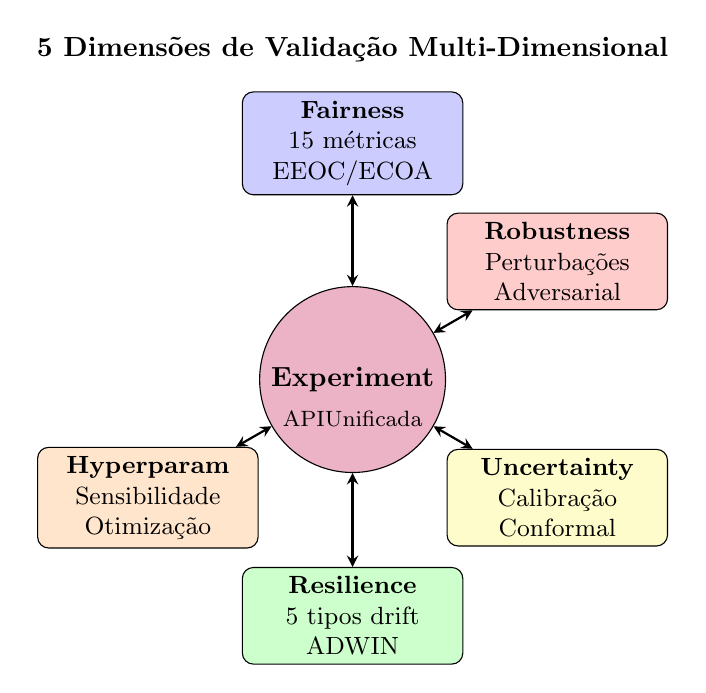
\begin{tikzpicture}[
    dimension/.style={rectangle, draw, rounded corners, minimum width=2.8cm, minimum height=1.2cm, align=center, font=\small, fill=#1},
    arrow/.style={->, >=stealth, thick}
]

% Central component
\node[circle, draw, fill=purple!30, minimum size=2cm, font=\bfseries] (exp) at (0,0) {Experiment};

% 5 dimensions around
\node[dimension=blue!20] (fairness) at (0,3) {\textbf{Fairness}\\15 métricas\\EEOC/ECOA};
\node[dimension=red!20] (robust) at (2.6,1.5) {\textbf{Robustness}\\Perturbações\\Adversarial};
\node[dimension=yellow!20] (uncertain) at (2.6,-1.5) {\textbf{Uncertainty}\\Calibração\\Conformal};
\node[dimension=green!20] (resilience) at (0,-3) {\textbf{Resilience}\\5 tipos drift\\ADWIN};
\node[dimension=orange!20] (hyperparam) at (-2.6,-1.5) {\textbf{Hyperparam}\\Sensibilidade\\Otimização};

% Arrows
\draw[arrow, <->] (exp) -- (fairness);
\draw[arrow, <->] (exp) -- (robust);
\draw[arrow, <->] (exp) -- (uncertain);
\draw[arrow, <->] (exp) -- (resilience);
\draw[arrow, <->] (exp) -- (hyperparam);

% Central label
\node[font=\footnotesize] at (0,-0.5) {API\\Unificada};

% Title
\node[font=\bfseries] at (0,4.2) {5 Dimensões de Validação Multi-Dimensional};

\end{tikzpicture}
\caption{As cinco dimensões de validação integradas no DeepBridge através de uma API unificada. Cada dimensão é gerenciada por um Test Manager especializado, coordenado pelo Experiment orchestrator.}
\label{fig:validation_dimensions}
\end{figure}


\begin{table}[htbp]
\centering
\caption{Dimensões de Validação Multi-Dimensional no DeepBridge}
\label{tab:validation_dimensions}
\small
\begin{tabular}{lllp{4cm}}
\toprule
\textbf{Dimensão} & \textbf{Foco} & \textbf{\# Métricas} & \textbf{Motivação} \\
\midrule
Fairness & Equidade & 15 & Compliance regulatório (EEOC, ECOA, GDPR) \\
Robustness & Perturbações & 10+ & Resiliência a ruído, ataques adversariais \\
Uncertainty & Confiança & 8 & Quantificação de incerteza para decisões críticas \\
Resilience & Drift & 5 tipos & Adaptação a mudanças de distribuição \\
Hyperparameters & Sensibilidade & N/A & Compreensão do impacto de configurações \\
\bottomrule
\end{tabular}
\end{table}

\paragraph{Motivação}
Modelos de ML em produção falham de formas distintas de software tradicional~\cite{sculley2015hidden}:
\begin{itemize}
    \item \textbf{Falhas silenciosas}: Degradação gradual sem alarmes explícitos
    \item \textbf{Falhas localizadas}: Bom desempenho global mas falhas em subgrupos específicos
    \item \textbf{Falhas emergentes}: Comportamentos inesperados em dados OOD (out-of-distribution)
\end{itemize}

Validação multi-dimensional detecta essas falhas através de testes complementares que cobrem diferentes aspectos de qualidade.

% ========================================
% 4.2 Fairness Suite
% ========================================

\subsection{Fairness Suite: Validação de Equidade}
\label{sec:validation:fairness}

A \textit{Fairness Suite} implementa 15 métricas de equidade categorizadas em três níveis: individual, grupo e causal. Esta suite é única por integrar verificação automática de compliance regulatório (detalhada na Seção~\ref{sec:compliance}).

\subsubsection{Taxonomia de Métricas}

\paragraph{Métricas de Nível Individual}
Garantem tratamento consistente de indivíduos similares~\cite{dwork2012fairness}:

\begin{itemize}
    \item \textbf{Individual Fairness}: $d(\mathbf{x}_i, \mathbf{x}_j) \leq \epsilon \Rightarrow |f(\mathbf{x}_i) - f(\mathbf{x}_j)| \leq \delta$

    Indivíduos com features similares (distância $\leq \epsilon$) devem receber predições similares (diferença $\leq \delta$).

    \item \textbf{Consistency}: Mede quão consistente é o modelo para vizinhos próximos no espaço de features:
    $$
    \text{Consistency} = 1 - \frac{1}{n} \sum_{i=1}^n \frac{|\{j \in kNN(i) : \hat{y}_j \neq \hat{y}_i\}|}{k}
    $$
    onde $kNN(i)$ são os $k$ vizinhos mais próximos de $i$.
\end{itemize}

\paragraph{Métricas de Nível Grupo}
Comparam resultados entre grupos protegidos e não-protegidos. Dado atributo sensível $S \in \{0, 1\}$ (e.g., $S=1$ para grupo protegido), target $Y$ e predição $\hat{Y}$:

\begin{enumerate}
    \item \textbf{Demographic Parity (Statistical Parity)}:
    $$
    P(\hat{Y} = 1 | S = 1) = P(\hat{Y} = 1 | S = 0)
    $$
    Taxa de predições positivas deve ser igual entre grupos.

    \item \textbf{Disparate Impact (4/5ths Rule)}:
    $$
    \text{DI} = \frac{P(\hat{Y} = 1 | S = 1)}{P(\hat{Y} = 1 | S = 0)}
    $$
    EEOC exige $\text{DI} \geq 0.80$ (regra dos 80\%)~\cite{eeoc1978uniform}.

    \item \textbf{Equal Opportunity}:
    $$
    P(\hat{Y} = 1 | Y = 1, S = 1) = P(\hat{Y} = 1 | Y = 1, S = 0)
    $$
    Taxa de verdadeiros positivos (recall) deve ser igual entre grupos.

    \item \textbf{Equalized Odds}:
    $$
    \begin{cases}
    P(\hat{Y} = 1 | Y = 1, S = 1) = P(\hat{Y} = 1 | Y = 1, S = 0) \\
    P(\hat{Y} = 1 | Y = 0, S = 1) = P(\hat{Y} = 1 | Y = 0, S = 0)
    \end{cases}
    $$
    Tanto TPR quanto FPR devem ser iguais entre grupos.

    \item \textbf{Predictive Parity}:
    $$
    P(Y = 1 | \hat{Y} = 1, S = 1) = P(Y = 1 | \hat{Y} = 1, S = 0)
    $$
    Precisão (PPV) deve ser igual entre grupos.

    \item \textbf{Calibration}:
    $$
    P(Y = 1 | \hat{p} = p, S = 1) = P(Y = 1 | \hat{p} = p, S = 0) = p
    $$
    onde $\hat{p}$ é a probabilidade predita. Modelo é calibrado se probabilidades refletem frequências reais.
\end{enumerate}

\paragraph{Métricas Causais}
Capturam causalidade através de intervenções contrafactuais~\cite{kusner2017counterfactual}:

\begin{itemize}
    \item \textbf{Counterfactual Fairness}:
    $$
    P(\hat{Y}_{\mathbf{x}, S \leftarrow s} | \mathbf{X} = \mathbf{x}, S = s) = P(\hat{Y}_{\mathbf{x}, S \leftarrow s'} | \mathbf{X} = \mathbf{x}, S = s)
    $$
    Predição não deve mudar ao intervir no atributo sensível $S$.

    \item \textbf{Path-Specific Fairness}: Decompõe efeitos em caminhos diretos e indiretos usando DAGs causais.
\end{itemize}

\subsubsection{Detecção de Weakspots}

DeepBridge implementa \textit{weakspot detection}~\cite{buolamwini2018gender}: identificação automática de subgrupos onde o modelo performa mal. Algoritmo:

\begin{algorithm}[htbp]
\caption{Weakspot Detection}
\label{alg:weakspot}
\begin{algorithmic}[1]
\STATE \textbf{Input:} Dataset $\mathcal{D}$, modelo $f$, threshold $\tau$, max depth $d$
\STATE \textbf{Output:} Lista de weakspots $W$
\STATE $W \leftarrow \emptyset$
\STATE $Q \leftarrow \{(\mathcal{D}, \text{``all data''})\}$ \COMMENT{Queue com (subset, descrição)}
\WHILE{$Q \neq \emptyset$ and depth $< d$}
    \STATE $(D_{subset}, desc) \leftarrow Q.\text{pop}()$
    \STATE $\text{acc} \leftarrow \text{accuracy}(f, D_{subset})$
    \IF{$\text{acc} < \tau$}
        \STATE $W \leftarrow W \cup \{(D_{subset}, desc, \text{acc})\}$
    \ENDIF
    \FOR{cada feature $f_i$ em $D_{subset}$}
        \STATE Particionar $D_{subset}$ em bins baseado em $f_i$
        \FOR{cada bin $b$}
            \STATE Adicionar $(b, desc + \text{`` AND } f_i \in b\text{''})$ a $Q$
        \ENDFOR
    \ENDFOR
\ENDWHILE
\RETURN $W$ ordenado por accuracy crescente
\end{algorithmic}
\end{algorithm}

Exemplo de output:
\begin{lstlisting}[caption=Weakspots detectados em modelo de crédito]
Weakspot 1: gender=Female AND age<25 AND income<30k
  - Size: 847 samples (2.3% of data)
  - Accuracy: 0.62 (vs 0.85 global)
  - Disparate Impact: 0.73 (FAIL)

Weakspot 2: race=Black AND debt_ratio>0.5
  - Size: 1,234 samples (3.4% of data)
  - Accuracy: 0.68
  - Equal Opportunity: 0.71 vs 0.89 (white group)
\end{lstlisting}

\subsubsection{API de Fairness Suite}

\begin{lstlisting}[language=Python, caption=Uso da Fairness Suite]
from deepbridge import DBDataset, Experiment

# Setup
dataset = DBDataset(data=df, target_column='approved', model=model,
                    protected_attributes=['gender', 'race', 'age'])

exp = Experiment(dataset, tests=['fairness'])

# Executar fairness tests
results = exp.run_tests(config='full')

# Resultados incluem:
# - 15 metricas de fairness
# - Verificacao automatica EEOC/ECOA
# - Weakspots detectados
# - Recomendacoes de mitigacao

print(results['fairness']['metrics']['disparate_impact'])
# {'gender': 0.82, 'race': 0.76, 'age': 0.91}

print(results['fairness']['compliance']['eeoc_80_rule'])
# {'gender': 'PASS', 'race': 'FAIL', 'age': 'PASS'}

# Gerar relatorio visual
exp.save_html('fairness', 'fairness_report.html')
\end{lstlisting}

% ========================================
% 4.3 Robustness Suite
% ========================================

\subsection{Robustness Suite: Testes de Robustez}
\label{sec:validation:robustness}

A \textit{Robustness Suite} avalia resiliência do modelo a perturbações, ataques adversariais e variações naturais dos dados. Implementa três categorias de testes:

\subsubsection{Testes de Perturbação}

Adição de ruído gaussiano/uniforme a features para avaliar estabilidade:

\begin{lstlisting}[language=Python, caption=Perturbation testing]
# Definir niveis de ruido
noise_levels = [0.05, 0.1, 0.2, 0.5, 1.0]

for sigma in noise_levels:
    # Adicionar ruido gaussiano
    X_noisy = X + np.random.normal(0, sigma, X.shape)

    # Avaliar degradacao
    acc_noisy = accuracy(model.predict(X_noisy), y)
    degradation = (acc_original - acc_noisy) / acc_original

    results[f'noise_{sigma}'] = {
        'accuracy': acc_noisy,
        'degradation': degradation
    }
\end{lstlisting}

Métricas reportadas:
\begin{itemize}
    \item \textbf{Robustness Score}: $R(\sigma) = 1 - \frac{\text{acc}_{\text{original}} - \text{acc}_{\sigma}}{\text{acc}_{\text{original}}}$
    \item \textbf{Noise Sensitivity}: Taxa de mudança $\frac{dR}{d\sigma}$
    \item \textbf{Critical Threshold}: Menor $\sigma$ onde $R(\sigma) < 0.90$
\end{itemize}

\subsubsection{Testes Adversariais}

DeepBridge implementa três ataques adversariais clássicos adaptados para dados tabulares~\cite{carlini2017towards}:

\paragraph{FGSM (Fast Gradient Sign Method)}
$$
\mathbf{x}_{adv} = \mathbf{x} + \epsilon \cdot \text{sign}(\nabla_{\mathbf{x}} \mathcal{L}(f(\mathbf{x}), y))
$$
onde $\mathcal{L}$ é a função de perda e $\epsilon$ é a magnitude da perturbação.

\paragraph{PGD (Projected Gradient Descent)}
Versão iterativa de FGSM com projeção em bola $L_\infty$:
$$
\mathbf{x}_{t+1} = \Pi_{\mathcal{B}_\epsilon(\mathbf{x})} \left( \mathbf{x}_t + \alpha \cdot \text{sign}(\nabla_{\mathbf{x}} \mathcal{L}(f(\mathbf{x}_t), y)) \right)
$$

\paragraph{Carlini \& Wagner (C\&W)}
Otimização de perturbação mínima:
$$
\min_{\delta} \|\delta\|_2 + c \cdot \max(0, f(\mathbf{x} + \delta)_y - \max_{i \neq y} f(\mathbf{x} + \delta)_i)
$$

Para dados tabulares, aplicamos restrições adicionais:
\begin{itemize}
    \item \textbf{Feature constraints}: Features categóricas não são perturbadas
    \item \textbf{Domain constraints}: Valores perturbados permanecem em domínios válidos (e.g., idade $\geq 0$)
    \item \textbf{Plausibility}: Perturbações respeitam correlações entre features
\end{itemize}

\subsubsection{Slice-Based Testing}

Avaliação em fatias (slices) específicas dos dados~\cite{chung2019slice}:

\begin{lstlisting}[language=Python, caption=Slice-based robustness testing]
# Definir slices de interesse
slices = {
    'low_income': df['income'] < 30000,
    'young': df['age'] < 25,
    'high_debt': df['debt_ratio'] > 0.5,
    'minority': df['race'].isin(['Black', 'Hispanic', 'Asian'])
}

for name, mask in slices.items():
    X_slice = X[mask]
    y_slice = y[mask]

    # Testar robustez neste slice
    results[name] = {
        'size': mask.sum(),
        'accuracy': accuracy(model.predict(X_slice), y_slice),
        'noise_sensitivity': compute_noise_sensitivity(X_slice, y_slice)
    }
\end{lstlisting}

% ========================================
% 4.4 Uncertainty Suite
% ========================================

\subsection{Uncertainty Suite: Quantificação de Incerteza}
\label{sec:validation:uncertainty}

A \textit{Uncertainty Suite} quantifica a confiança do modelo em suas predições, crítico para decisões de alto impacto onde incerteza deve ser comunicada.

\subsubsection{Calibration}

Verifica se probabilidades preditas refletem frequências reais~\cite{guo2017calibration}. Métrica principal:

\paragraph{Expected Calibration Error (ECE)}
$$
\text{ECE} = \sum_{m=1}^M \frac{|B_m|}{n} \left| \text{acc}(B_m) - \text{conf}(B_m) \right|
$$
onde $B_m$ são bins de probabilidades, $\text{acc}(B_m)$ é accuracy no bin e $\text{conf}(B_m)$ é confiança média.

DeepBridge também calcula:
\begin{itemize}
    \item \textbf{Maximum Calibration Error (MCE)}: $\max_m |\text{acc}(B_m) - \text{conf}(B_m)|$
    \item \textbf{Static Calibration Error}: Weighted ECE
    \item \textbf{Adaptive Calibration Error}: Bins adaptativos por quantis
\end{itemize}

Visualização via reliability diagram:
\begin{lstlisting}[language=Python, caption=Reliability diagram]
exp.plot_reliability_diagram(save_path='calibration.png')
# Plota accuracy vs confidence em bins
# Linha diagonal = calibracao perfeita
\end{lstlisting}

\subsubsection{Conformal Prediction}

Implementa predição conformal~\cite{vovk2005algorithmic} para intervalos de predição com garantias de cobertura:

\paragraph{Split Conformal Prediction}
\begin{algorithm}[htbp]
\caption{Split Conformal Prediction}
\begin{algorithmic}[1]
\STATE \textbf{Input:} Calibration set $\mathcal{D}_{cal}$, modelo $f$, nível $\alpha$
\STATE Computar non-conformity scores: $s_i = |y_i - f(\mathbf{x}_i)|$ para $(\mathbf{x}_i, y_i) \in \mathcal{D}_{cal}$
\STATE $\hat{q} \leftarrow (1 - \alpha)$-quantil de $\{s_i\}$
\STATE \textbf{Para novo} $\mathbf{x}_{test}$:
\STATE \quad $\hat{y} = f(\mathbf{x}_{test})$
\STATE \quad \textbf{Return} $[\hat{y} - \hat{q}, \hat{y} + \hat{q}]$ \COMMENT{Intervalo com cobertura $\geq 1-\alpha$}
\end{algorithmic}
\end{algorithm}

Garantia: $P(y_{test} \in [\hat{y} - \hat{q}, \hat{y} + \hat{q}]) \geq 1 - \alpha$ para qualquer distribuição.

DeepBridge suporta:
\begin{itemize}
    \item \textbf{Split CP}: Divisão simples calibration/test
    \item \textbf{Cross-Conformal}: CV-based para datasets pequenos
    \item \textbf{Adaptive CP}: Intervalos adaptativos por região
\end{itemize}

\subsubsection{Uncertainty Decomposition}

Para modelos probabilísticos, DecompBridge decompõe incerteza em:

\paragraph{Aleatoric Uncertainty (Epistemic)}
Incerteza inerente aos dados, irredutível:
$$
\mathbb{E}_{\mathbf{x}}[H(P(y|\mathbf{x}))]
$$
onde $H$ é entropia.

\paragraph{Epistemic Uncertainty}
Incerteza devido a conhecimento limitado do modelo, redutível com mais dados:
$$
H(\mathbb{E}_{\mathbf{x}}[P(y|\mathbf{x})]) - \mathbb{E}_{\mathbf{x}}[H(P(y|\mathbf{x}))]
$$

Implementação via ensemble ou dropout Bayesiano:
\begin{lstlisting}[language=Python, caption=Uncertainty decomposition]
from deepbridge.uncertainty import UncertaintyDecomposition

decomp = UncertaintyDecomposition(model, method='ensemble', n_models=10)
aleatoric, epistemic = decomp.decompose(X_test)

# High epistemic: Modelo incerto, coletar mais dados
# High aleatoric: Incerteza inerente, melhorar features
\end{lstlisting}

% ========================================
% 4.5 Resilience Suite
% ========================================

\subsection{Resilience Suite: Detecção de Drift}
\label{sec:validation:resilience}

A \textit{Resilience Suite} monitora mudanças na distribuição dos dados ao longo do tempo, detectando cinco tipos de drift~\cite{gama2014survey}:

\subsubsection{Tipos de Drift}

\paragraph{1. Data Drift (Covariate Shift)}
Mudança na distribuição de features: $P_{train}(\mathbf{X}) \neq P_{prod}(\mathbf{X})$

Detecção via:
\begin{itemize}
    \item \textbf{Population Stability Index (PSI)}:
    $$
    \text{PSI} = \sum_{i=1}^k (P_{prod}^i - P_{train}^i) \ln\left(\frac{P_{prod}^i}{P_{train}^i}\right)
    $$
    Thresholds: PSI $< 0.1$ (estável), $0.1$-$0.25$ (monitorar), $> 0.25$ (drift significativo)

    \item \textbf{Kolmogorov-Smirnov (KS)}: Para features contínuas:
    $$
    D_{KS} = \sup_x |F_{train}(x) - F_{prod}(x)|
    $$
\end{itemize}

\paragraph{2. Concept Drift}
Mudança na relação $P(Y|\mathbf{X})$: mesmo input leva a outputs diferentes.

\paragraph{3. Label Drift}
Mudança na distribuição de labels: $P_{train}(Y) \neq P_{prod}(Y)$

\paragraph{4. Prediction Drift}
Mudança na distribuição de predições: $P(\hat{Y})$ muda ao longo do tempo.

\paragraph{5. Feature Drift}
Mudança em features individuais detectada por testes estatísticos.

\subsubsection{Pipeline de Detecção}

\begin{lstlisting}[language=Python, caption=Pipeline de detecção de drift]
from deepbridge.resilience import DriftDetector

# Configurar detector
detector = DriftDetector(
    reference_data=X_train,  # Baseline
    drift_types=['data', 'concept', 'prediction'],
    test='psi',  # ou 'ks', 'chi2', 'wasserstein'
    threshold=0.1
)

# Monitorar producao
for batch in production_batches:
    drift_report = detector.detect(batch)

    if drift_report.has_drift:
        print(f"Drift detectado: {drift_report.drifted_features}")
        print(f"Severidade: {drift_report.severity}")
        # Acionar retreinamento ou alertas
\end{lstlisting}

\subsubsection{Adaptive Windowing}

DeepBridge implementa ADWIN (ADaptive WINdowing)~\cite{bifet2007learning} para detecção adaptativa de drift:

\begin{itemize}
    \item Mantém janela deslizante de tamanho variável
    \item Detecta mudanças significativas na média da janela
    \item Reduz janela quando drift é detectado
\end{itemize}

% ========================================
% 4.6 Hyperparameter Sensitivity Suite
% ========================================

\subsection{Hyperparameter Sensitivity Suite}
\label{sec:validation:hyperparameters}

A \textit{Hyperparameter Sensitivity Suite} analisa como hiperparâmetros do modelo afetam desempenho e fairness, identificando configurações robustas.

\subsubsection{Sensitivity Analysis}

\paragraph{Sobol Sensitivity Analysis}
Decompõe variância em contribuições de hiperparâmetros individuais e interações:

$$
\text{Var}(Y) = \sum_i V_i + \sum_{i<j} V_{ij} + \ldots + V_{12\ldots k}
$$

onde $V_i$ é variância devido ao hiperparâmetro $i$ e $V_{ij}$ é efeito de interação.

Índices de sensibilidade:
\begin{itemize}
    \item \textbf{First-order}: $S_i = V_i / \text{Var}(Y)$
    \item \textbf{Total-order}: $S_T^i = \sum_{j: i \in j} V_j / \text{Var}(Y)$ (inclui interações)
\end{itemize}

\subsubsection{Multi-Objective Optimization}

Encontra configurações que balanceiam accuracy e fairness:

\begin{lstlisting}[language=Python, caption=Multi-objective hyperparameter optimization]
from deepbridge.hyperparameters import MultiObjectiveOptimizer

# Definir espacos de busca
param_space = {
    'max_depth': [3, 5, 10, 15],
    'min_samples_split': [2, 5, 10],
    'class_weight': ['balanced', None]
}

# Otimizar
optimizer = MultiObjectiveOptimizer(
    objectives=['accuracy', 'disparate_impact'],
    constraints={'disparate_impact': ('>=', 0.80)}  # EEOC compliance
)

pareto_front = optimizer.optimize(param_space, X_train, y_train)

# Resultado: Conjunto de configuracoes nao-dominadas
# Usuario escolhe tradeoff desejado
\end{lstlisting}

\subsubsection{Robustness to Hyperparameters}

Avalia quão sensível o modelo é a pequenas mudanças nos hiperparâmetros:

$$
\text{HP-Robustness} = \frac{1}{|\Theta|} \sum_{\theta \in \Theta} \exp\left(-\frac{\|\text{acc}(\theta) - \text{acc}(\theta_0)\|^2}{\sigma^2}\right)
$$

onde $\Theta$ é vizinhança de $\theta_0$ e $\sigma$ controla tolerância.

% ========================================
% 4.7 Integração Multi-Suite
% ========================================

\subsection{Integração Multi-Suite}
\label{sec:validation:integration}

Uma das principais contribuições do DeepBridge é a capacidade de executar múltiplas suites de forma integrada, detectando trade-offs entre dimensões:

\begin{lstlisting}[language=Python, caption=Validação multi-dimensional integrada]
# Executar todas as 5 suites
exp = Experiment(dataset, tests='all')
results = exp.run_tests(config='full')

# Analise de trade-offs
print("=== TRADE-OFF ANALYSIS ===")
print(f"Accuracy: {results['metrics']['accuracy']:.3f}")
print(f"Fairness (DI): {results['fairness']['disparate_impact']:.3f}")
print(f"Robustness (noise 0.2): {results['robustness']['noise_0.2']:.3f}")
print(f"Calibration (ECE): {results['uncertainty']['ece']:.3f}")
print(f"Drift (PSI): {results['resilience']['psi_mean']:.3f}")

# Gerar relatorio completo
exp.save_pdf('all', 'comprehensive_validation.pdf')
\end{lstlisting}

\paragraph{Detecção de Trade-offs}
DeepBridge automaticamente identifica trade-offs:
\begin{itemize}
    \item \textbf{Accuracy vs. Fairness}: Modelos com maior accuracy podem ter pior fairness
    \item \textbf{Robustness vs. Accuracy}: Defesas adversariais podem reduzir accuracy
    \item \textbf{Calibration vs. Accuracy}: Modelos bem calibrados podem ter menor accuracy
\end{itemize}

% ========================================
% 4.8 Sumário
% ========================================

\subsection{Sumário}
\label{sec:validation:summary}

O framework de validação multi-dimensional do DeepBridge oferece:

\begin{enumerate}
    \item \textbf{Cobertura abrangente}: 5 dimensões, 40+ métricas individuais
    \item \textbf{API unificada}: Interface consistente para todas as suites
    \item \textbf{Integração automática}: Detecção de trade-offs entre dimensões
    \item \textbf{Production-ready}: Testes otimizados para datasets grandes (>100GB)
    \item \textbf{Compliance-aware}: Verificação automática de requisitos regulatórios
\end{enumerate}

A Tabela~\ref{tab:validation_summary} resume as capacidades de cada suite.

\begin{table}[htbp]
\centering
\caption{Resumo das Suites de Validação}
\label{tab:validation_summary}
\small
\begin{tabular}{llll}
\toprule
\textbf{Suite} & \textbf{Métricas} & \textbf{Tempo (est.)} & \textbf{Escalável >1GB} \\
\midrule
Fairness & 15 & 5-15 min & \cmark \\
Robustness & 10+ & 10-30 min & \cmark \\
Uncertainty & 8 & 5-10 min & \cmark \\
Resilience & 5 tipos & 2-5 min & \cmark \\
Hyperparameters & N/A & 30-120 min & $\triangle$ \\
\bottomrule
\multicolumn{4}{l}{\footnotesize \cmark: Completo; $\triangle$: Parcial (requer amostragem)}
\end{tabular}
\end{table}

A próxima seção (Seção~\ref{sec:compliance}) detalha o \textit{Compliance Engine}, que automatiza verificação de requisitos regulatórios (EEOC, ECOA, GDPR) sobre as métricas de fairness.
